\documentclass{ximera}

\newcommand{\RR}{\mathbb R}
\renewcommand{\d}{\,d}
\newcommand{\dd}[2][]{\frac{d #1}{d #2}}
\renewcommand{\l}{\ell}
\newcommand{\ddx}{\frac{d}{dx}}
\newcommand{\dfn}{\textbf}
\newcommand{\eval}[1]{\bigg[ #1 \bigg]}


%% The launch should somehow present a ``mystery'' for the students to
%% solve.  Moreover, it should lead them to the right path. Ideally if
%% we had a bright student working on the launch, they might even
%% develop the techniques from the lesson to solve the problem.  By
%% the end of the lesson, the mystery is solved!

\outcome{Understand the meaning of the inputs and outputs of a position function.}
\outcome{Compute average velocity using a position function.}
\outcome{Understand the connection between average velocity and instantaneous velocity.}
\outcome{Express instantaneous velocity as a limit of average velocities.}


\title[Break-Ground:]{From average velocity to instantaneous velocity}

\begin{document}

\begin{abstract}
Building from a single example, we develop the background for
derivatives.
\end{abstract}
\maketitle

%% Here the idea is to be truthful, enthuastic, and narrow. We want a
%% SINGLE example. So for this prototype we could talk about all kinds
%% of rates of change, but lets refrain from this.


Let me tell you about something that is really awesome:
\href{http://en.wikipedia.org/wiki/Global_Positioning_System}{The
  Global Positioning System.} 
  %STEVE SAYS:  I do not think we should be linking directly to a pdf here.
  Seriously, this is a modern ``Wonder of
the World.'' With this system, the secrets of navigating our beautiful
blue sphere are no longer limited to an elite few. Instead we have
devices small enough to fit in our pockets, that cost as little as a
few meals, that can tell us where we are, and even \textit{how fast we
  are going.} Think about this, in World War II, a GPS in the right
(or wrong) hands would have been powerful enough to change the course
of history!

While the details of how GPS works are fascinating, incorporating many
concepts from mathematics and physics, including
\href{relativisticEffectsInTheGlobalPositioningSystem.pdf}{Einstein's
  theory of relativity}, what we are most interested in is how a GPS
computes velocity from position.

The \textit{MOOCulus Team} recently took a road trip from Columbus
Ohio to Urbana-Champaign Illinois in the \textit{MOOCulus-Mobile}:
\begin{image}
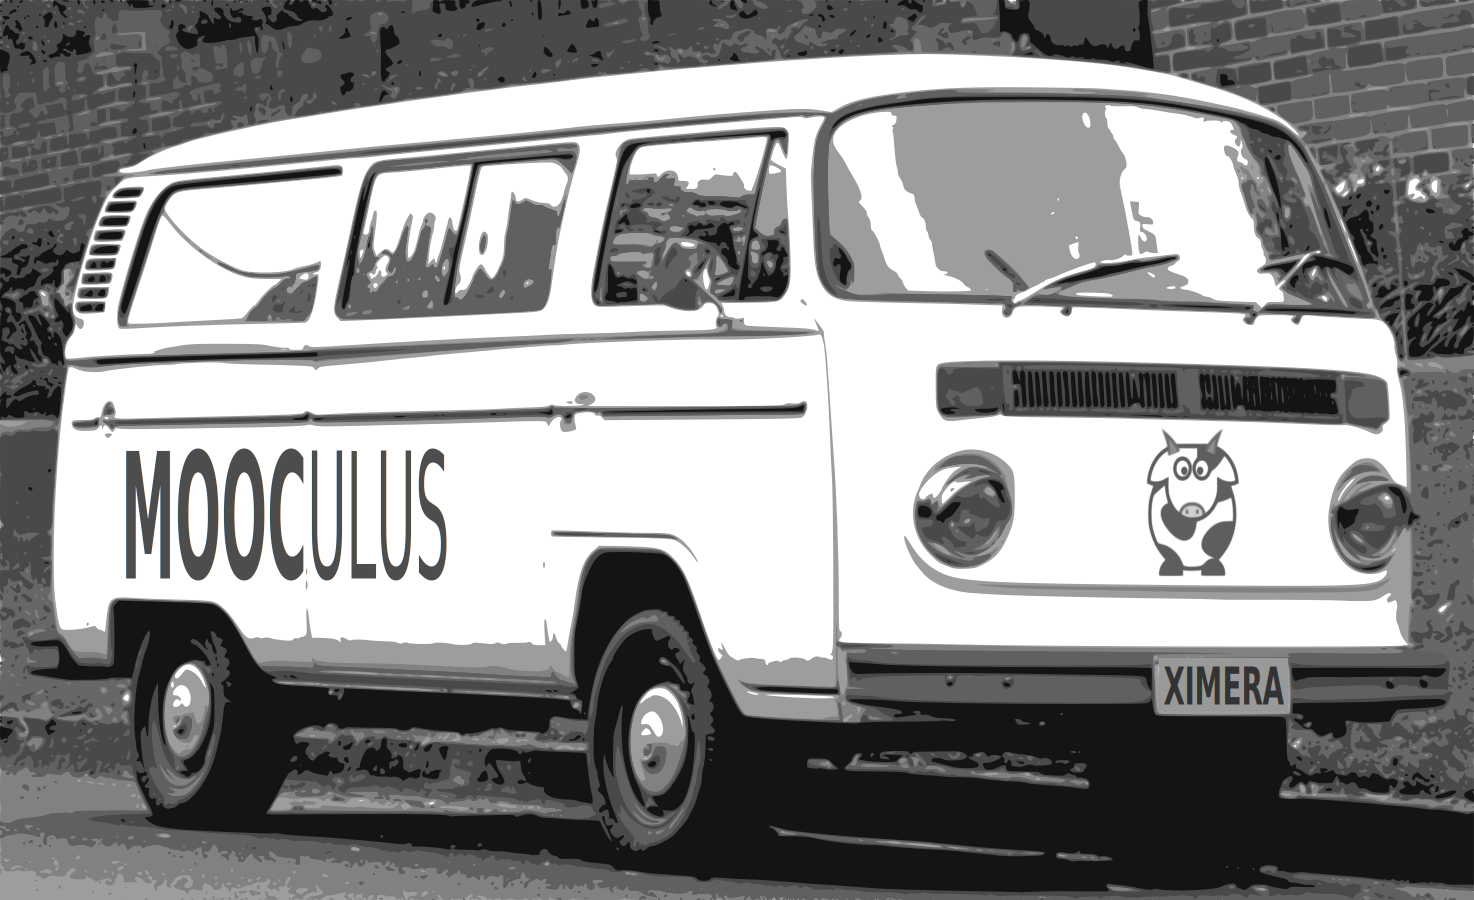
\includegraphics[width=3in]{mooculusMobile.pdf} %% http://commons.wikimedia.org/wiki/File:1973-1980_Volkswagen_Kombi_(T2)_van_01.jpg
\end{image}
While the MOOCulus-Mobile might look pretty spiffy, it has some
quirks, in particular, it has no speedometer!  Never-to-be-flustered,
the MOOCulus team can use their GPS to compute the velocity. To see
how this works, we need some background. Urbana-Champaign is around
$300$ miles dead West of Columbus. The position of the MOOCulus-Mobile
is roughly modeled by
\[
s(t) = 36t^2 -4.8t^3 \qquad\text{(miles West of Columbus)} %% note the model is wrong
\]
where $t$ is measured in hours. 

\begin{problem} %% Here we are asking the student to think about context
What does $s(0)$ correspond to in terms of the context of our road
trip?
\begin{hint}
Remember $s(t)$ is position at time $t$.
\end{hint}
\begin{hint}
So $s(0)$ is where you are after no time has passed.
\end{hint}
\begin{prompt} %% note the use of prompt here
  \begin{multipleChoice}
    \choice[correct]{Our starting point, Columbus Ohio.}
    \choice{Our ending point, Urbana-Champaign Illinois.}
    \choice{Ann-Arbor Michigan, because the MOOCulus Team got lost.}
  \choice{There is no way to be certain.}
  \end{multipleChoice}
\end{prompt}
\end{problem}

\begin{problem} %% Here we are asking the student to think about context
If $b$ corresponds to the time where $s(b) = 300$, what does $b$ mean
in terms of the context of our road trip?
\begin{hint}
Remember $s(t)$ is position at time $t$.
\end{hint}
\begin{hint}
So $s(b)=300$ is a statement relating time and position.  
\end{hint}
\begin{prompt} %% note the use of prompt here
  \begin{multipleChoice}
    \choice[correct]{$b$ is how many hours it takes the MOOCulus Team to travel to Urbana-Champaign.} 
    \choice{$b$ is the time the MOOCulus Team arrives after noon.}
    \choice{$b$ is the time the MOOCulus Team arrives after midnight.}
    \choice{There is no way to be certain.}
  \end{multipleChoice}
\end{prompt}
\end{problem}


\begin{problem} %% A VERY important problem
Consider again the function that roughly models the position of the
MOOCulus-Mobile
\[
s(t) = 36t^2 - 4.8t^3.
\]
Assuming the final destination is Urbana-Champaign Illinois, on what
domain does this model make sense?
\begin{hint}
  Plot $s(t)$ and choose the domain that makes sense in the context of
  the problem.
\end{hint}
\end{problem}

\begin{problem}
  What is the average velocity for the MOOCulus-Mobile for the entire trip? 
\begin{hint}
  Remember, 
  \[
  \text{change in distance} = \text{rate}\cdot\text{change in time}.
  \]
\end{hint}
\begin{hint}
  So, 
  \[
  \frac{\Delta\text{distance}}{\Delta\text{time}} = \text{rate}.
  \]
\end{hint}
\begin{hint}
So, 
\[
\frac{\Delta\text{distance}}{\Delta\text{time}} = \frac{300}{5}.
\]
\end{hint}
\begin{prompt}
  The average velocity is \answer{60} miles per hour.
\end{prompt}
\end{problem}

%STEVE SAYS: The stuff about I_h  kind of comes out of nowhere.  It might be better to ask questions in "natural language" in 
%this section, and add in the I_h notation in "Dig in", or even in "Reinforce".  We run the risk of losing the idea
%of "taking average rates of change over successively smaller intervals" if the student does not understand one of the
%following:  1. Using h as a variable. 2. Using a variable to define an interval. 3. Giving a variable name to an interval
% 4. How subscripts work in mathematics.  5.  How piecewise defined functions work. 6.  That a function can give an interval
% as an output.  Any one of these confusions could trip the student up here, and then they never get to think about
% average velocity over small intervals.  So I think just asking something like "What is the average rate of change
% on the interval [2,2.1]? [2,2.01]?  [1.999,2]?  Then introduce the variable h, mention that it can be positive or negative.
%We can even ask "What is the formula for the average rate of change when h is positive?" and then when it is negative.
%They should, of course, get the same answer.  If you want to discuss this more, let me know in a Trello comment, we can 
%chat.  I am happy to make these changes if you want.

Now let's get a bit crazy, consider this interval:
\[
I_h = 
\begin{cases}
  [2+h,2]  & \text{if $h<0$}, \\ %% note this is MORE correct than std books
  [2,2+h]  & \text{if $0<h$}.     %% in the content section, we can explain this in detail
\end{cases}
\]

%% For these next problems using h=0.5 and h=-0.5 is intentional. 

\begin{problem}
  What is this interval when $h = 0.5$?
\todo{We need an answer-type for intervals}
\end{problem}

\begin{problem}
  What is the average velocity of the MOOCulus-Mobile on $I_h$ when $h =
  0.5$?
  \begin{prompt} %% note the use of prompt here
    \answer{88.8} miles per hour.
  \end{prompt}
\end{problem}

\begin{problem}
  What is this interval when $h = -0.5$?
\todo{We need an answer-type for intervals}
\end{problem}

\begin{problem}
  What is the average velocity of the MOOCulus-Mobile on $I_h$ when $h =
  -0.5$?
  \begin{prompt} %% note the use of prompt here
    \answer{81.6} miles per hour.
  \end{prompt}
\end{problem}

\begin{problem}
  Write a formula that will compute the average velocity of the
  MOOCulus-Mobile at $t=2$ hours for all given values of $h$.
\begin{hint}
Remember
\[
\frac{\Delta\text{distance}}{\Delta\text{time}} = \text{rate}.
\]
\end{hint}
\begin{hint}
So the average velocity is
\[
\frac{s(2+h)-s(2)}{h}.
\]
\end{hint}
\answer{(36*(2+h)^2 - 4.8*(2+h)^3 - (36*2^2 - 4.8*2^3))/h}
\end{problem}

Computing average velocities for smaller, and smaller, values of $h$ as
we did above is tedious. Nevertheless, this is exactly how a GPS
determines velocity from position! On the other hand, we are human
beings and have better things to do than just compute all day
long. What would really help us out is a formula.

\begin{problem}
  Given a formula for position, say $s(t) = 36t^2 -4.8t^3$, how do we
  find a formula for velocity?  Think about the previous problem and
  what we have done previously in the course.
  \begin{freeResponse}
  %Do we want a model solution here?  Maybe we only want them to be able to view a model solution after they submit something?
  \end{freeResponse} 
\end{problem}

\begin{xarmaBoost}
  Write down at least \textbf{five} questions for this lecture. After
you have your questions, label them as ``Level 1,'' ``Level 2,'' or ``Level 3'' where:
\begin{description}
\item[Level 1] Means you know the answer, or know exactly how to do
  this problem.
\item[Level 2] Means you think you know how to do the problem, or will
  soon learn how to do the problem.
\item[Level 3] Means you have no idea how to do the problem.
\end{description}
\begin{freeResponse}
\end{freeResponse}
\end{xarmaBoost}

\end{document}
